\section{Experiments}

\subsection{Implementation Details}

We conducted fine-tuning experiments on three model variants: \textit{Qwen3-VL-2B-Instruct} \cite{qwen2}, \textit{Qwen3-VL-4B-Instruct} \cite{qwen4}, and \textit{Qwen3-VL-8B-Instruct} \cite{qwen8}. The training configuration was kept consistent across all models to ensure a fair comparison.

All models were fine-tuned using Low-Rank Adaptation (LoRA) \cite{lora}, applied to the query, key, and value projection layers within the attention mechanisms \cite{attention}. We used the AdamW \cite{adam} optimizer with a learning rate of \(5 \times 10^{-4}\) and a cosine learning rate scheduler with a 5\% linear warmup phase \cite{warmup}.

Training was performed for 3 epochs on a single node equipped with 8 H100 GPUs. We utilized the Fully Sharded Data Parallel (FSDP) \cite{fsdp} strategy for efficient memory usage and distributed training, with a global batch size of 128.

The training loss curves for all model sizes are provided in \Cref{fig:loss}, demonstrating stable convergence over the course of training.

\begin{figure}[t]
    \centering
    
\includegraphics[width=\columnwidth]{loss.png}
    \caption{Learning curves for the fine-tuned models.}
    \label{fig:loss}
\end{figure}

\subsection{Quantitative Results}


\begin{table*}[t]
    \caption{Qualitative Results. Representative examples from fine-tuned and zero-shot models, illustrating differences in geometric complexity, artifact prevalence, and contextual adaptation.}
    \label{tab:qualitative}
    \centering
    \begin{tabular}{m{2cm} m{2cm} m{2cm} | m{2cm} m{2cm} m{2cm} | m{2cm}}
        \toprule
        \multicolumn{3}{c}{\thead{Input}} & \multicolumn{3}{c}{\thead{Output (fine-tuned)}} & \multicolumn{1}{c}{\thead{Output (zero-shot)}} \\ 
        \cmidrule(lr){1-3} \cmidrule(lr){4-6} \cmidrule(lr){7-7}
        \thead{Requirements} & \thead{Context} & \thead{Ground Truth} & \thead{CoMa-2B} & \thead{CoMa-4B} & \thead{CoMa-8B} & \thead{Qwen3-VL-235B} \\
        \midrule
        \adjustbox{valign=c, max width=2cm}{%
            \begin{tabular}{@{}l@{}}
                Building function: \\ \textit{Educational/Research} \\
                Floors count: \textit{15} \\
                Total area: \textit{15565} \\
                Dwellings count: \textit{0} \\
                Offices count: \textit{47} \\
                Offices public capacity: \textit{68} \\
            \end{tabular}%
        }
        &
        \centering\adjustbox{valign=c}{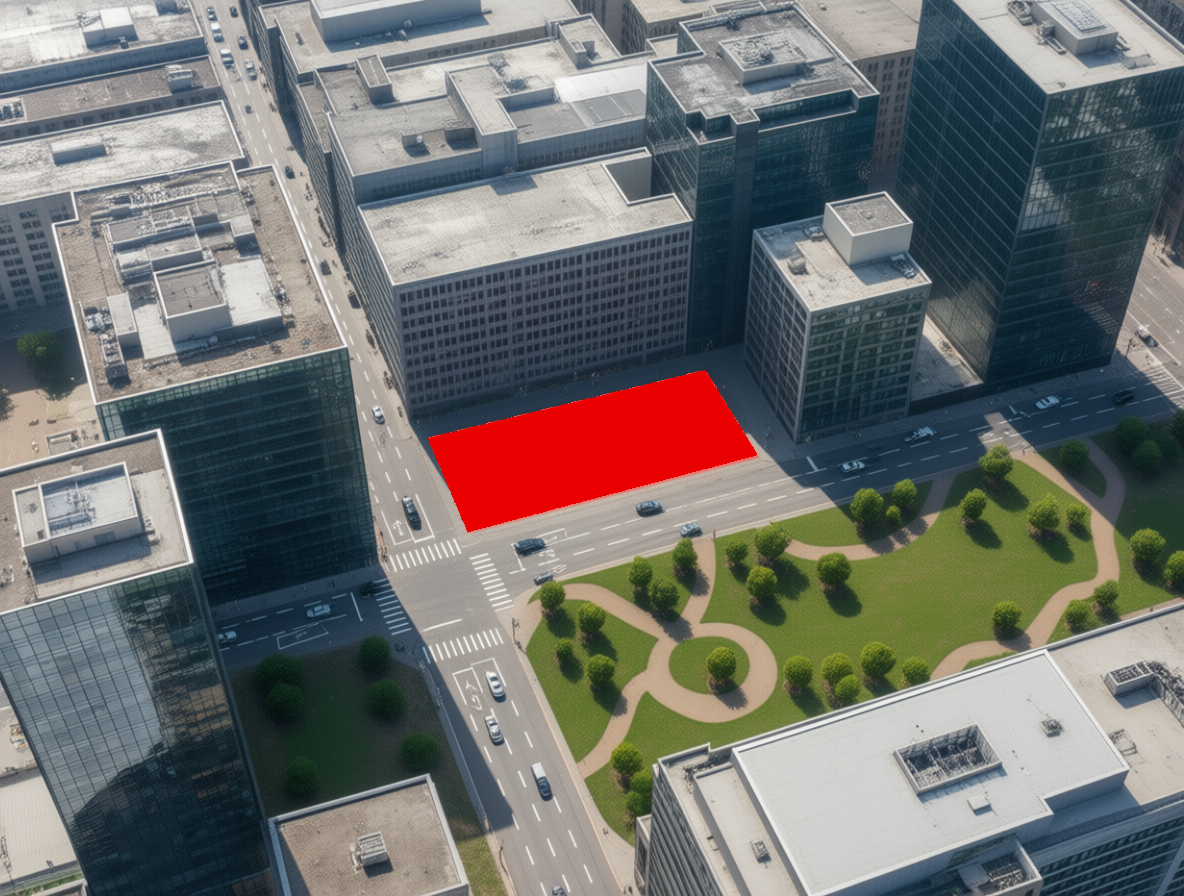
\includegraphics[width=1.9cm, frame]{images_samples_context_313.png}}
        &
        \centering\adjustbox{valign=c}{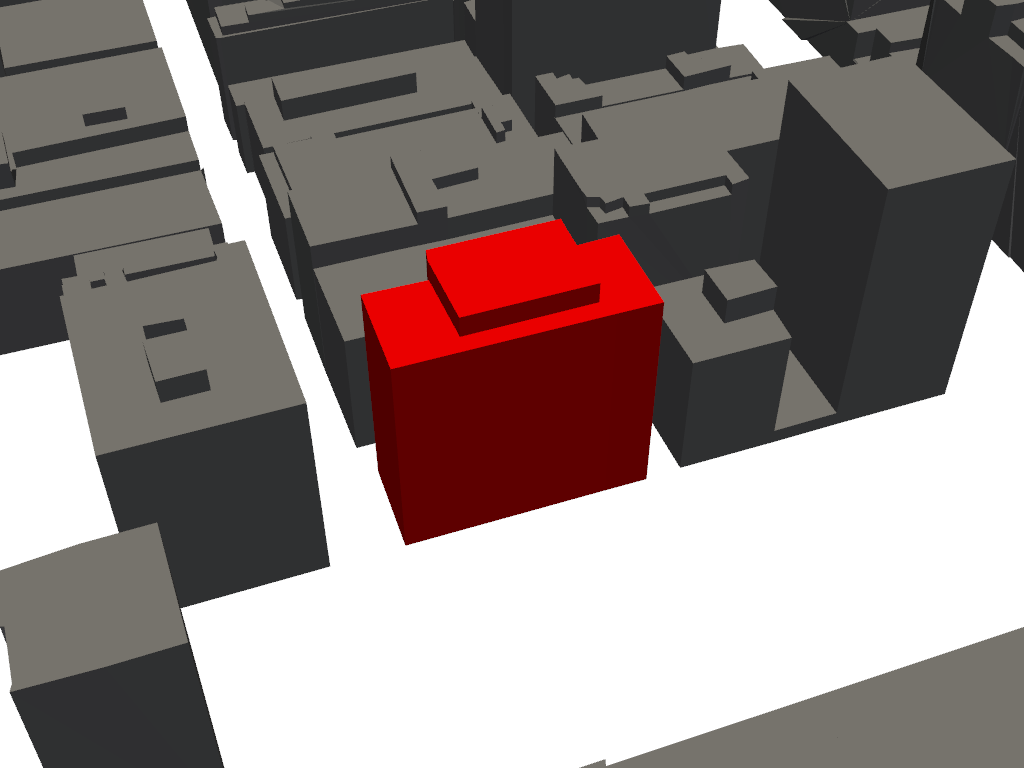
\includegraphics[width=1.9cm, frame]{images_samples_gt_313.png}}
        &
        \centering\adjustbox{valign=c}{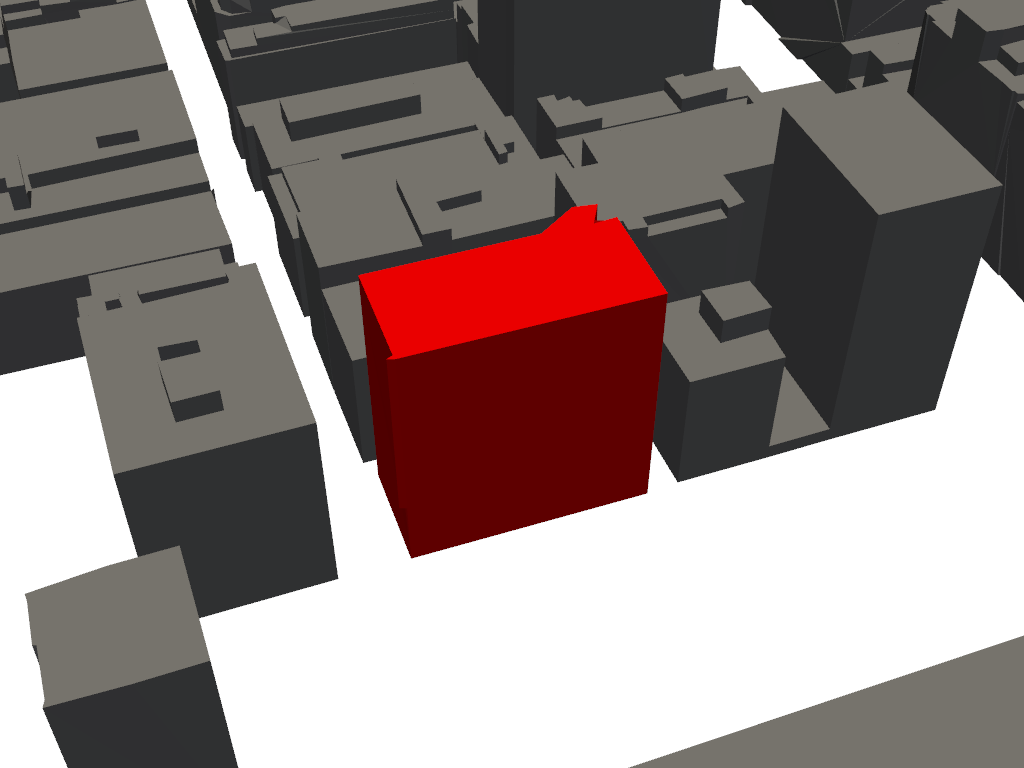
\includegraphics[width=1.9cm, frame]{images_samples_CoMa-2B_313.png}}
        &
        \centering\adjustbox{valign=c}{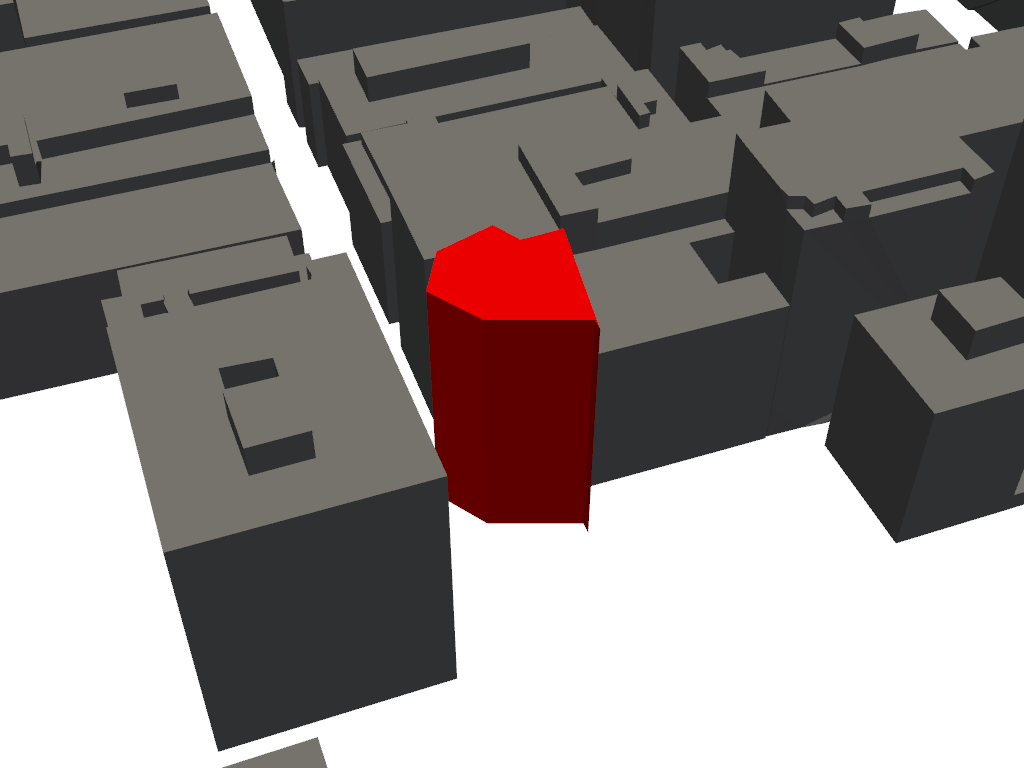
\includegraphics[width=1.9cm, frame]{images_samples_CoMa-4B_313.png}}
        &
        \centering\adjustbox{valign=c}{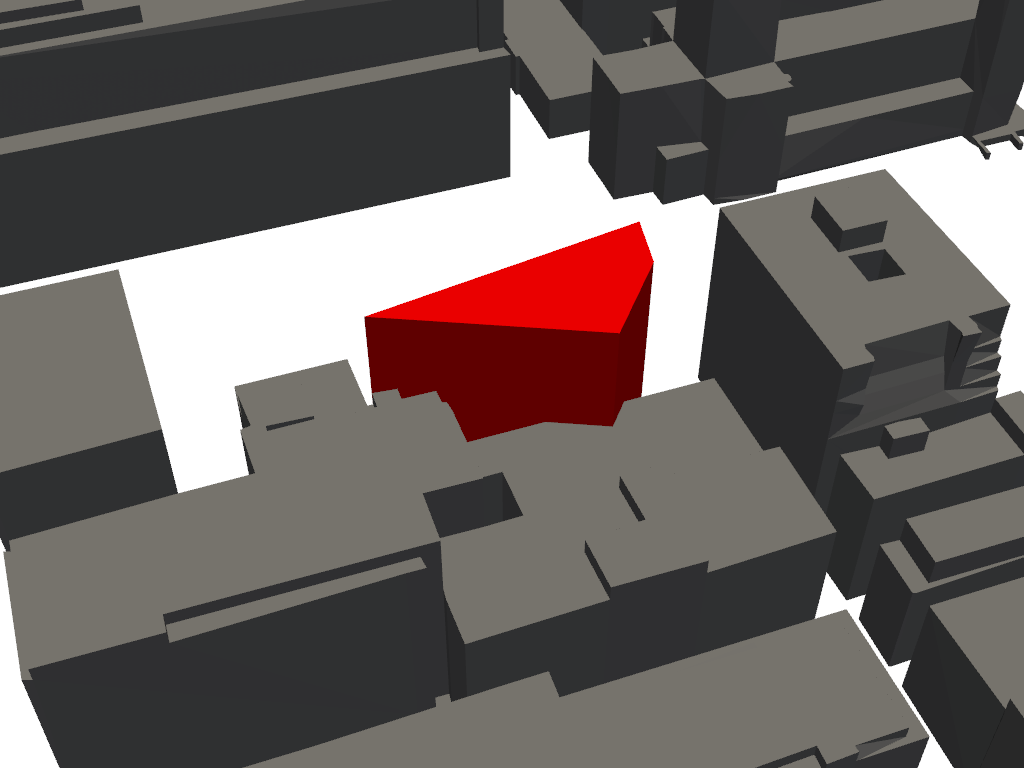
\includegraphics[width=1.9cm, frame]{images_samples_CoMa-8B_313.png}}
        &
        \adjustbox{valign=c}{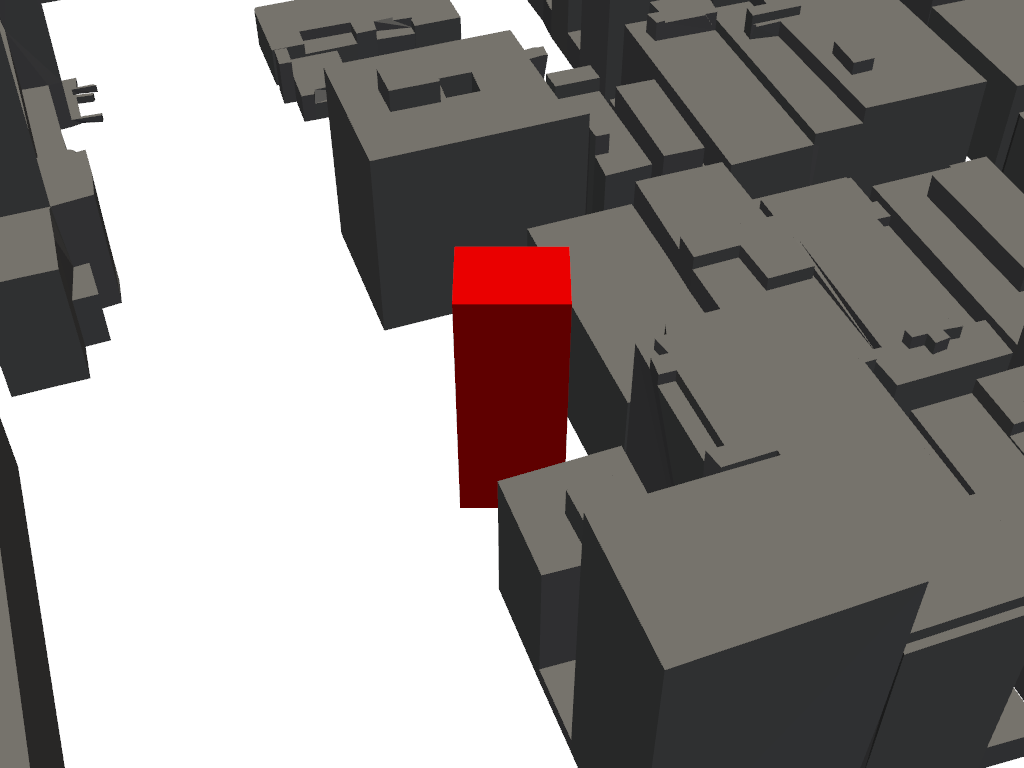
\includegraphics[width=1.9cm, frame]{images_samples_Qwen_313.png}} \\

        \midrule

        \adjustbox{valign=c, max width=2cm}{%
            \begin{tabular}{@{}l@{}}
                Building function: \\ \textit{Student Accommodation} \\
                Floors count: \textit{3} \\
                Total area: \textit{1551} \\
                Dwellings count: \textit{65} \\
                Offices count: \textit{0} \\
                Offices public capacity: \textit{0} \\
            \end{tabular}%
        }
        &
        \centering\adjustbox{valign=c}{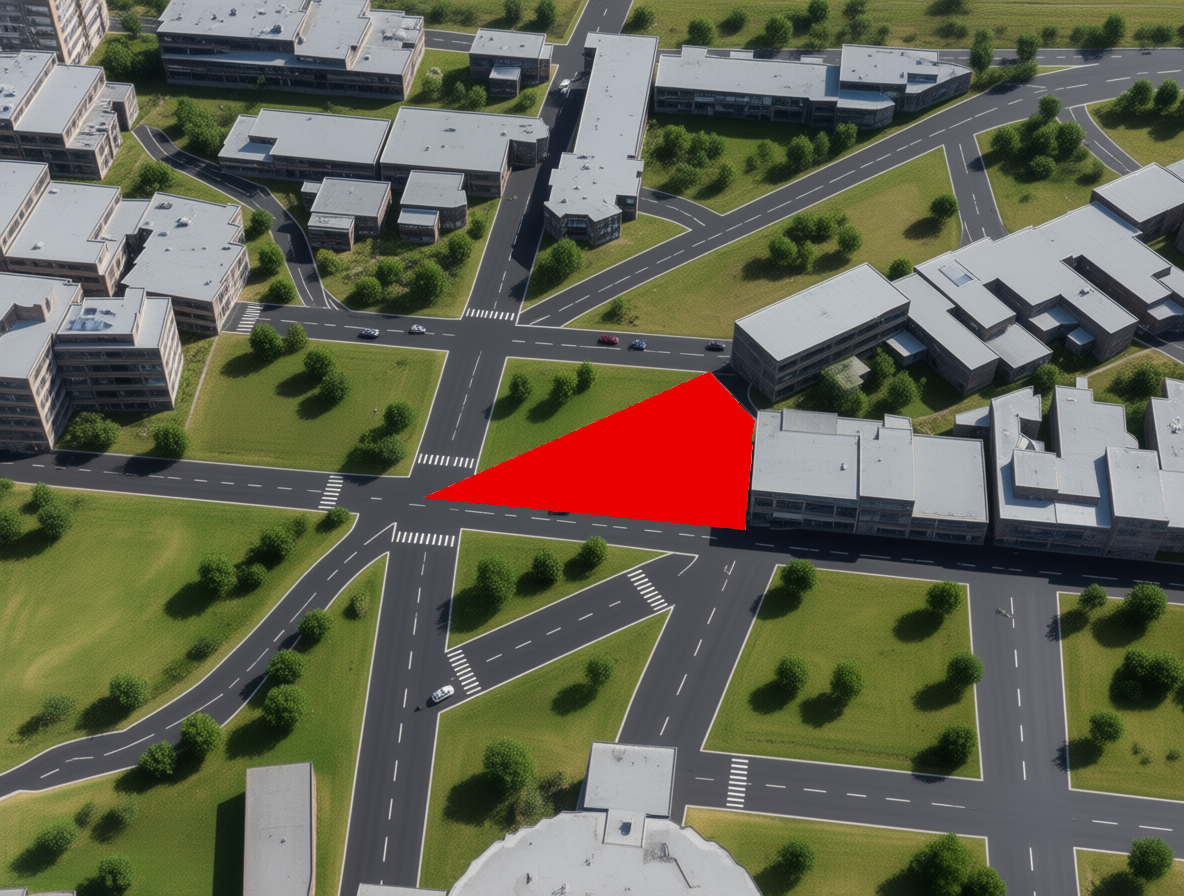
\includegraphics[width=1.9cm, frame]{images_samples_context_524.png}}
        &
        \centering\adjustbox{valign=c}{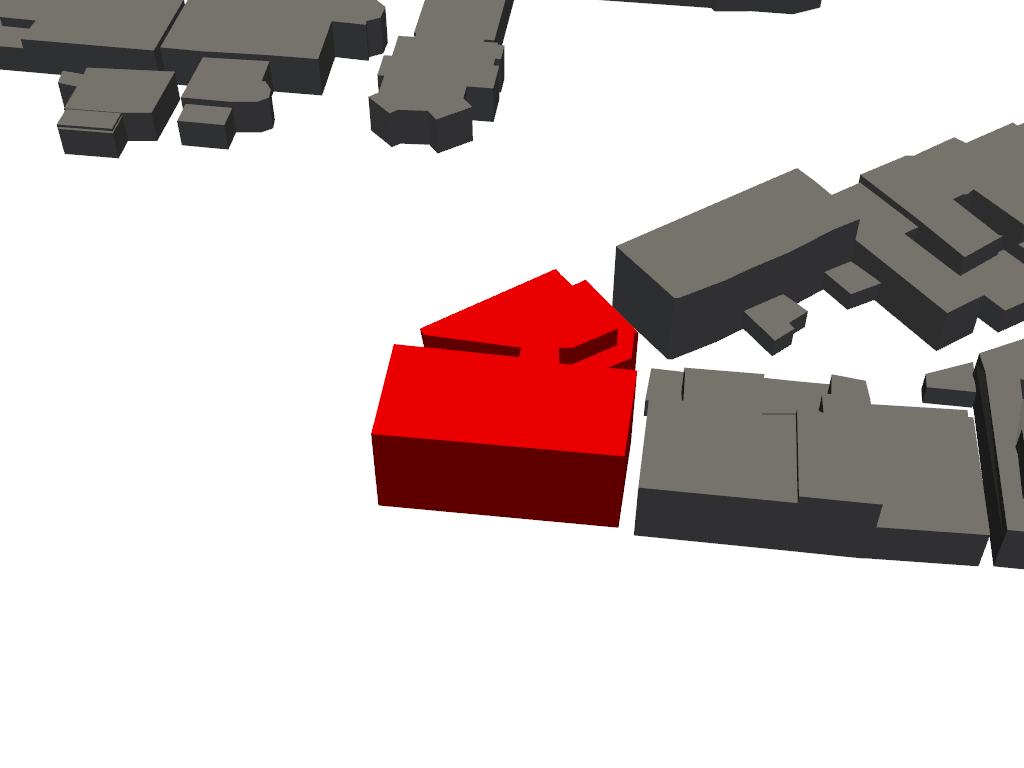
\includegraphics[width=1.9cm, frame]{images_samples_gt_524.png}}
        &
        \centering\adjustbox{valign=c}{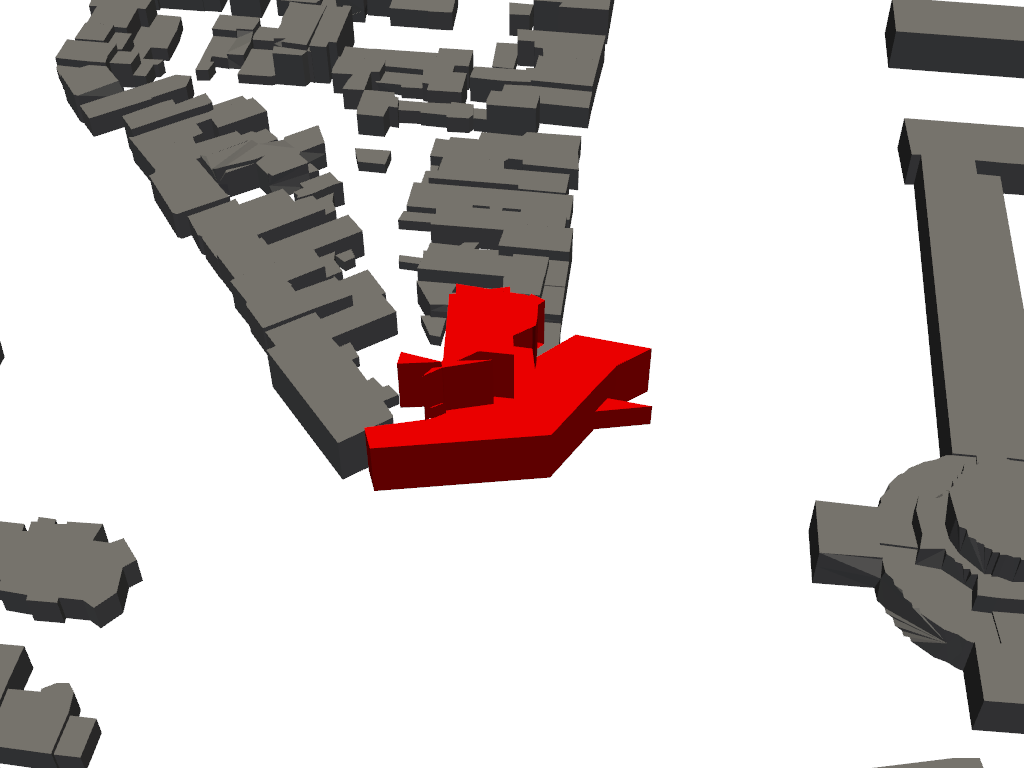
\includegraphics[width=1.9cm, frame]{images_samples_CoMa-2B_524.png}}
        &
        \centering\adjustbox{valign=c}{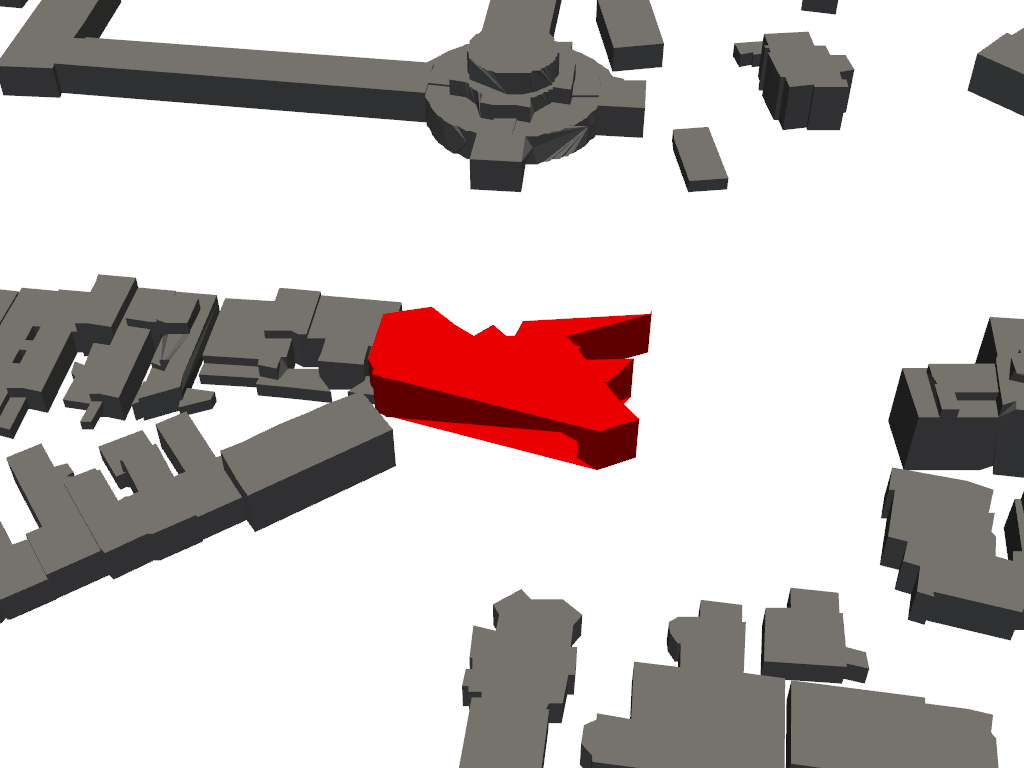
\includegraphics[width=1.9cm, frame]{images_samples_CoMa-4B_524.png}}
        &
        \centering\adjustbox{valign=c}{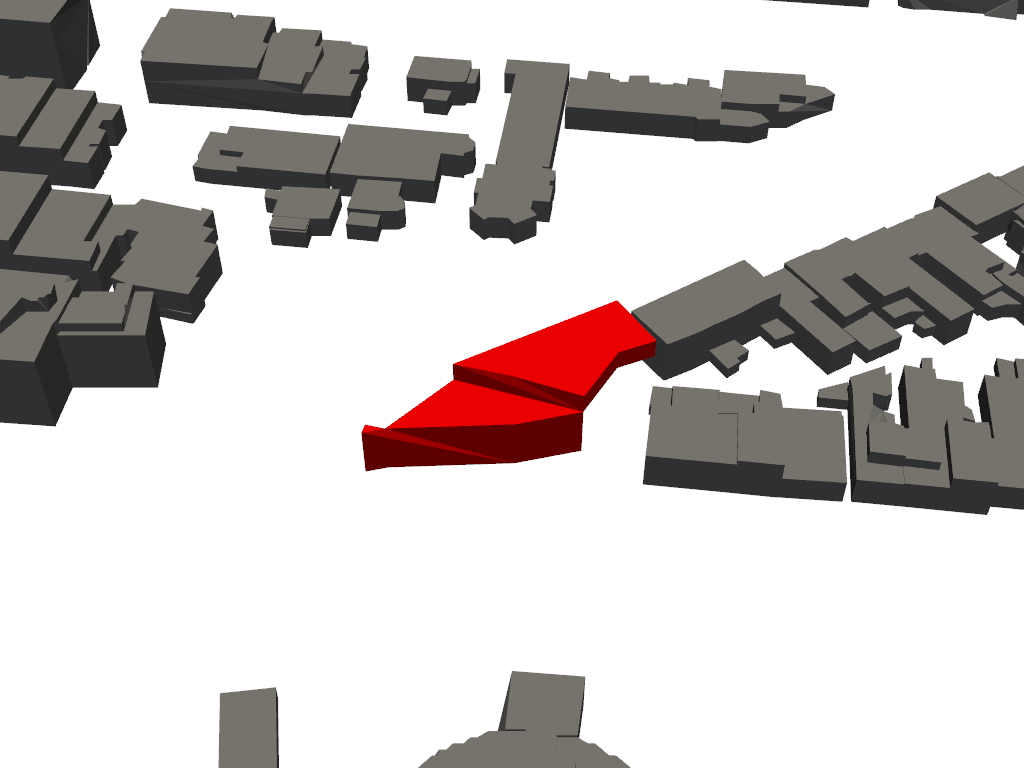
\includegraphics[width=1.9cm, frame]{images_samples_CoMa-8B_524.png}}
        &
        \adjustbox{valign=c}{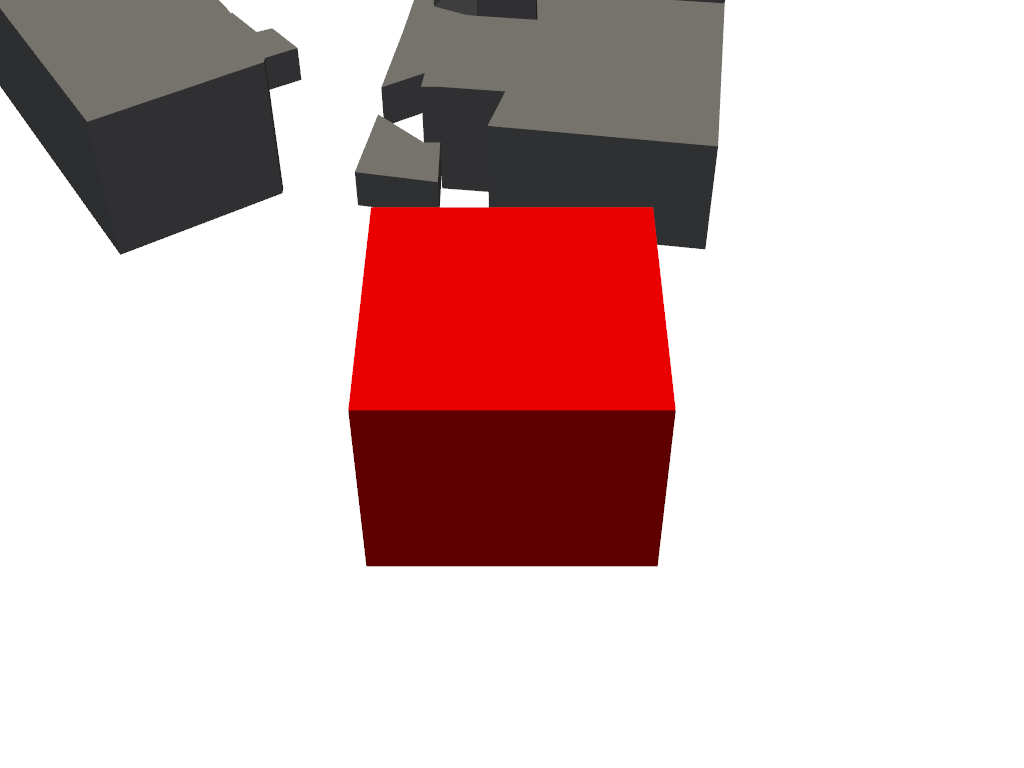
\includegraphics[width=1.9cm, frame]{images_samples_Qwen_524.png}} \\

        \midrule

        \adjustbox{valign=c, max width=2cm}{%
            \begin{tabular}{@{}l@{}}
                Building function: \\ \textit{Residential Apartment} \\
                Floors count: \textit{50} \\
                Total area: \textit{36259} \\
                Dwellings count: \textit{227} \\
                Offices count: \textit{4} \\
                Offices public capacity: \textit{0} \\
            \end{tabular}%
        }
        &
        \centering\adjustbox{valign=c}{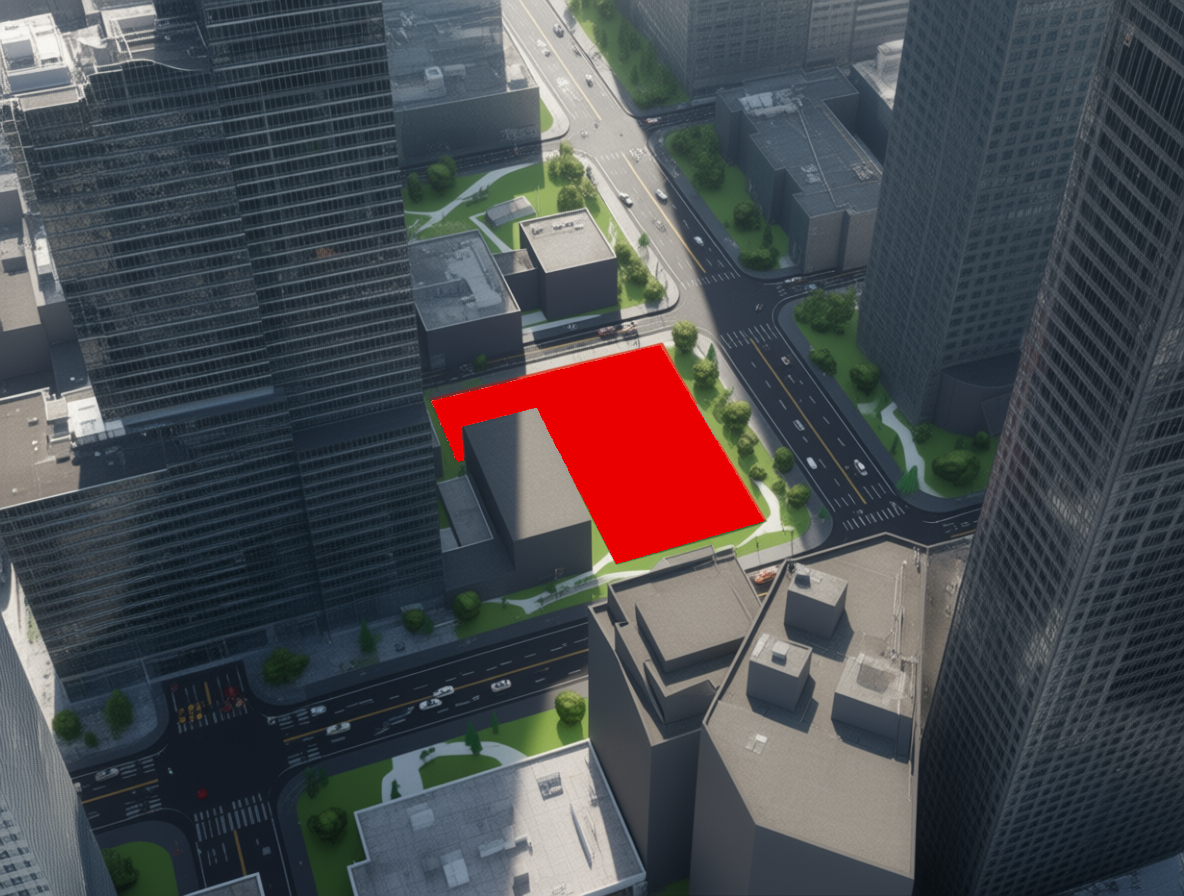
\includegraphics[width=1.9cm, frame]{images_samples_context_8041.png}}
        &
        \centering\adjustbox{valign=c}{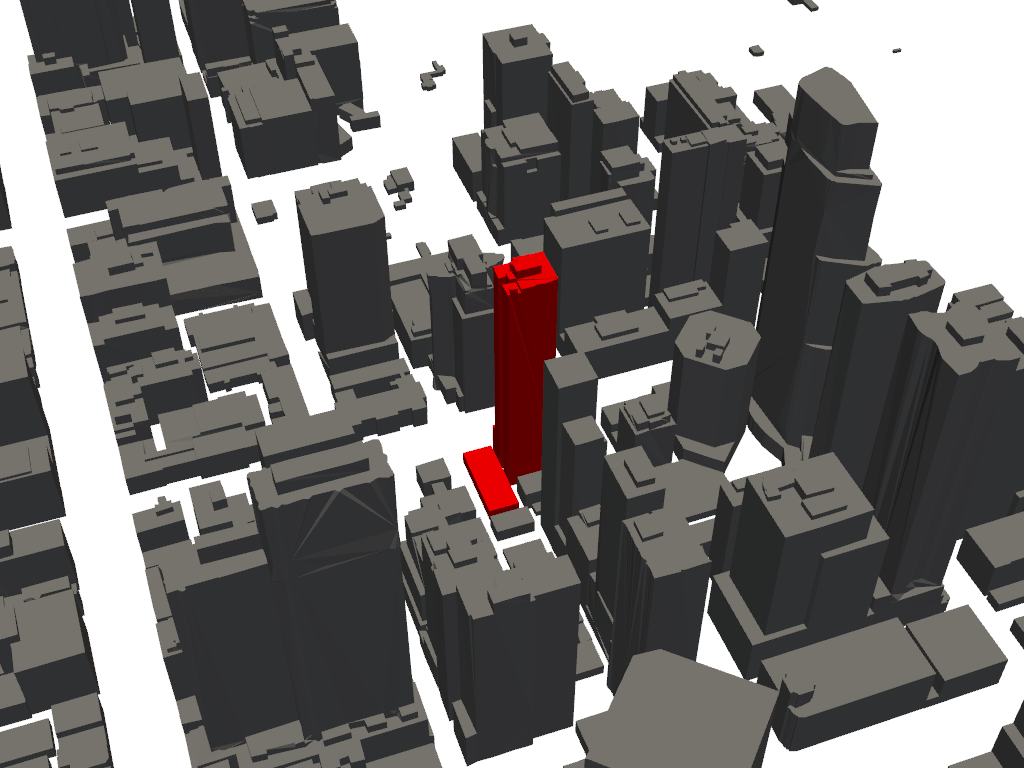
\includegraphics[width=1.9cm, frame]{images_samples_gt_8041.png}}
        &
        \centering\adjustbox{valign=c}{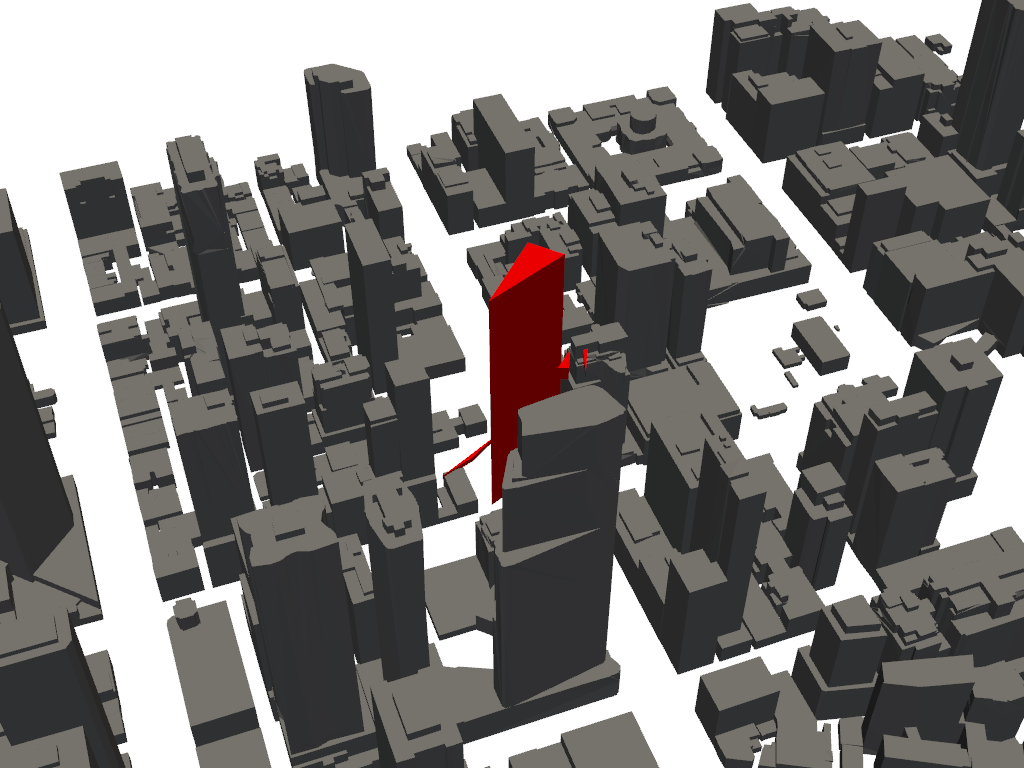
\includegraphics[width=1.9cm, frame]{images_samples_CoMa-2B_8041.png}}
        &
        \centering\adjustbox{valign=c}{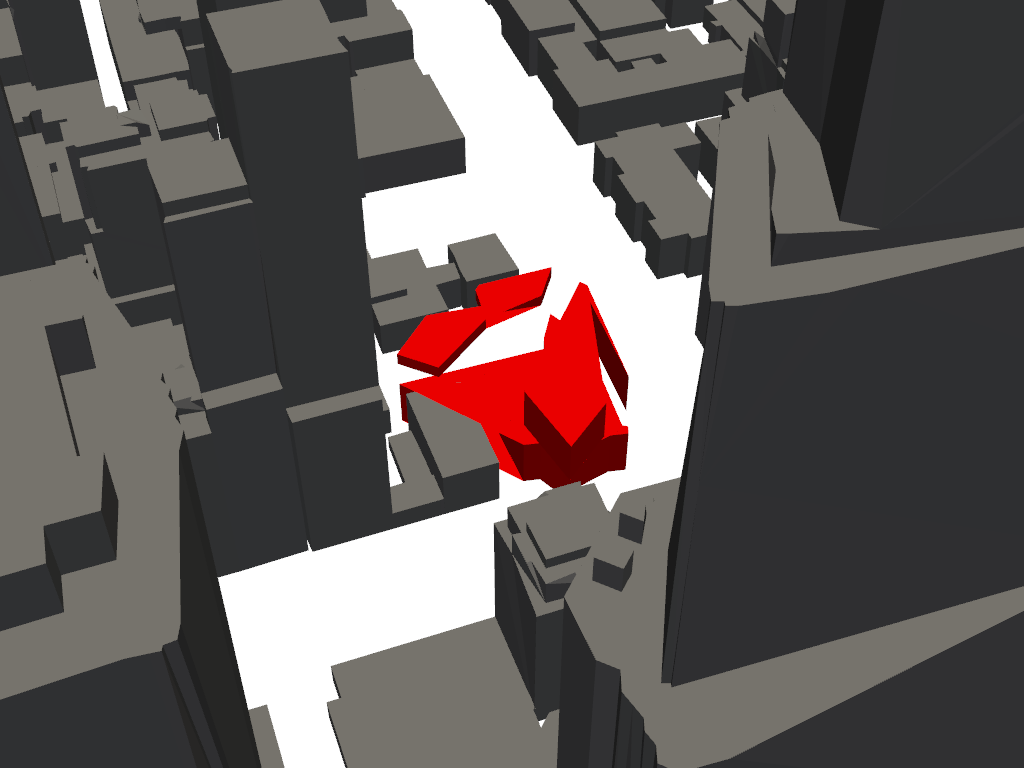
\includegraphics[width=1.9cm, frame]{images_samples_CoMa-4B_8041.png}}
        &
        \centering\adjustbox{valign=c}{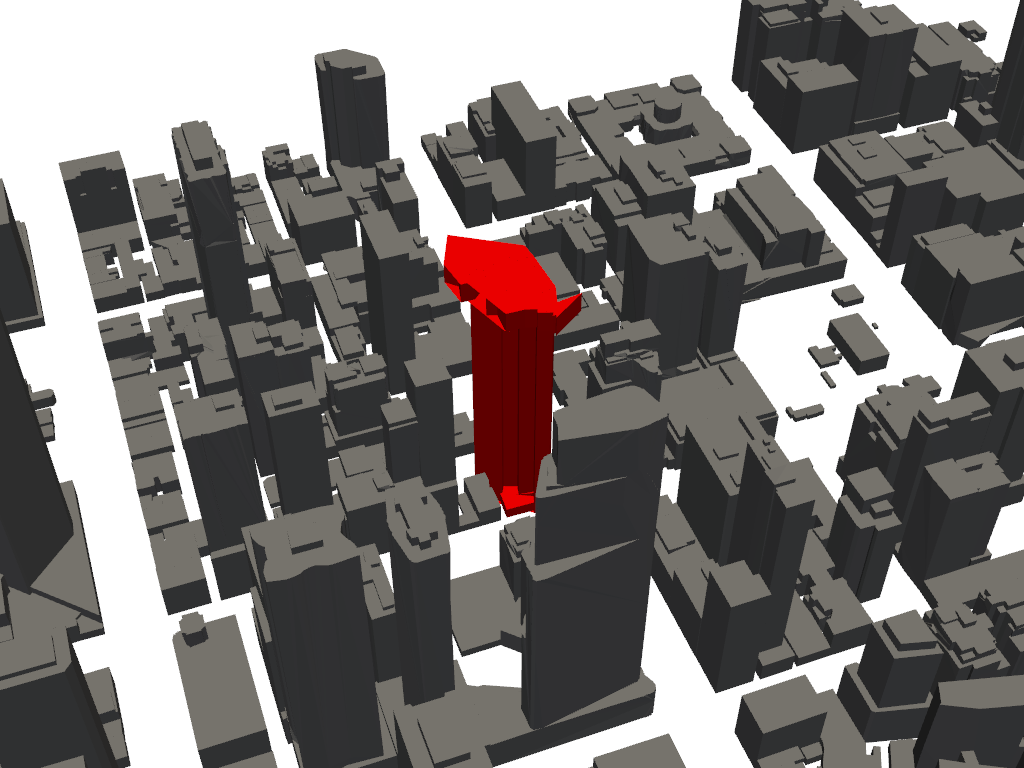
\includegraphics[width=1.9cm, frame]{images_samples_CoMa-8B_8041.png}}
        &
        \adjustbox{valign=c}{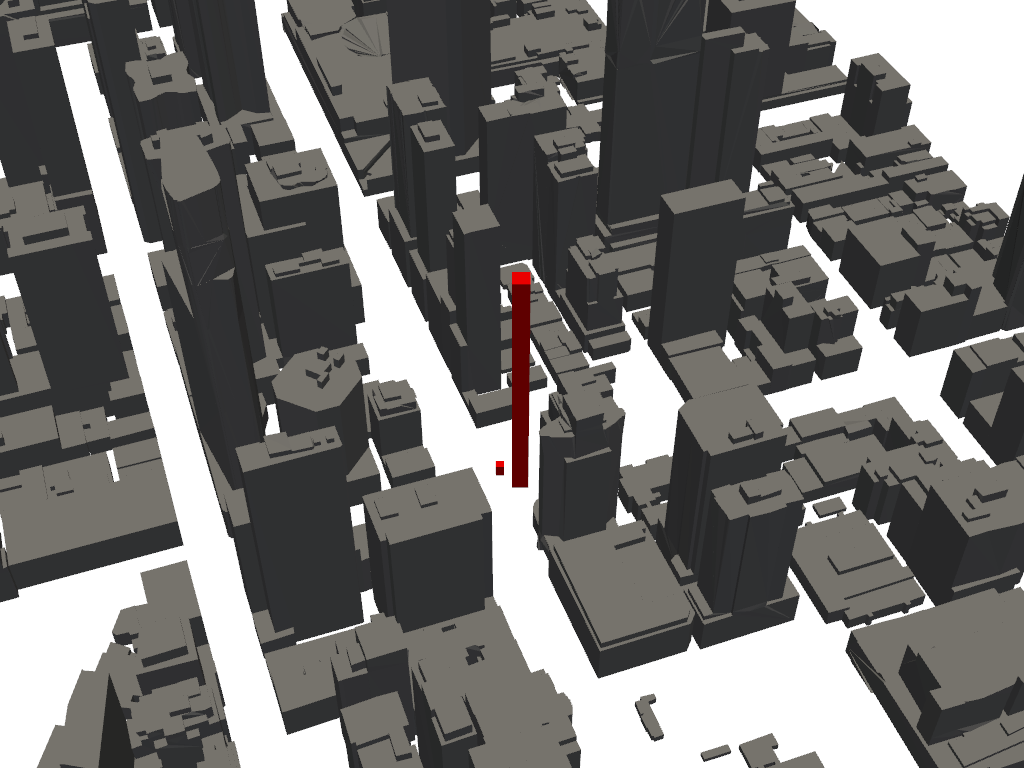
\includegraphics[width=1.9cm, frame]{images_samples_Qwen_8041.png}} \\
        
        \bottomrule
    \end{tabular}
\end{table*}

We evaluate both fine-tuned and zero-shot models using a comprehensive set of metrics designed to assess both the structural correctness and contextual appropriateness of the generated massings. The metrics are defined as follows:

\begin{itemize}
    \item \textbf{Pattern Match:} The rate of model outputs from which a JSON-like string can be successfully extracted.
    \item \textbf{JSON Validity:} The rate of extracted strings that are valid, parseable JSON.
    \item \textbf{ID IoU:} The Intersection-over-Union between the set of building IDs in the requirements and the set of IDs in the generated massing.
    \item \textbf{Floor Error:} The mean absolute difference between the required and predicted number of floors, averaged per site and normalized by the ground truth value. For a site with \(N\) buildings, it is computed as:
    \begin{equation}
        \frac{1}{N} \sum_{i=1}^{N} \frac{|F_{pred}^i - F_{gt}^i|}{F_{gt}^i}
        \label{eq:floor_error}
    \end{equation}
    \item \textbf{Area Error:} The mean absolute difference between the required and predicted usable area, averaged per site and normalized by the ground truth area:
    \begin{equation}
        \frac{1}{N} \sum_{i=1}^{N} \frac{|A_{pred}^i - A_{gt}^i|}{A_{gt}^i}
        \label{eq:area_error}
    \end{equation}
    \item \textbf{Site IoU:} The IoU between the ground truth site contour and the union of the bottom polygons of all generated buildings.
    \item \textbf{Contextual Relevance:} A binary score (0/1) assigned by a powerful VLM-as-a-judge (\textit{Qwen3-VL-235B-A22B-Thinking} \cite{qwen_think}), prompted with architectural rules to determine if the generated massing is plausible within its surrounding environment.
\end{itemize}

The quantitative results, presented in \Cref{tab:metrics}, reveal several key findings. Among the fine-tuned models, the largest 8B parameter model outperforms smaller models across all metrics except Area Error, where the 2B model achieves the best performance. The large zero-shot model demonstrates superior capability compared to small fine-tuned models, achieving near-perfect scores in format-related metrics (Pattern Match and JSON Validity) and showing competitive performance in Floor Error and Area Error. However, despite outperforming all fine-tuned models in Site IoU and Contextual Relevance, the absolute scores for these spatial and contextual metrics remain relatively low, indicating significant challenges in geometric accuracy and contextual integration that persist across all approaches.

\subsection{Qualitative Results}

Qualitative analysis of the generated massings reveals distinct behavioral patterns between the fine-tuned and zero-shot approaches. As shown in \Cref{tab:qualitative}, the fine-tuned models demonstrate a tendency to generate geometrically complex massings, often featuring articulated forms with multiple extrusions and varied roof heights. However, these complex outputs frequently contain geometric artifacts such as self-intersecting polygons and irregular shapes that deviate from architecturally plausible forms. This phenomenon can be attributed to the dataset's composition: while containing some highly complex examples, the CoMa-20K dataset is dominated by simpler massings, creating an imbalance that challenges the models' ability to generalize effectively for complex geometric generation.

In contrast, the large zero-shot model produces geometrically clean and consistent outputs, but exhibits strong limitations in complexity and contextual adaptation. The generated massings are predominantly simple rectangular forms with uniform orientations, demonstrating insufficient consideration of site contour geometry and surrounding building context. This suggests that while the model possesses strong general reasoning capabilities, it lacks specialized geometric understanding and fails to adequately incorporate spatial and contextual cues from the visual input, resulting in massings that, while structurally valid, are architecturally simplistic and contextually disconnected.

